\subsubsection{System.AddIn}
\label{sec:system_addin}

Разработка компании {\it Microsoft}, так же известеная под именем {\tt Managed AddIn Framework}~\cite{System.Addins-article, maf}. {\tt System.Addin} - это пространство имён {\tt(namespace)}, которое появилось в .NET Framework 3.5. По сути своей {\tt System.Addin} предоставляет разработчикам программную модель для расширения функционала приложения. Причём применение этой программной модели даёт несколько ключевых возможностей:

\begin{itemize}

  \item Хост-приложение и {\tt Addin} могут иметь независимые версии. Таким образом можно построить хост-приложение, которое бы работало и со сборками расширения, которые были построены для предыдущих версий приложения, либо для более поздних версий приложения, либо которые вообще были построены для другого приложения;

  \item Возможность активировать {\tt Addin} с нужным уровнем изоляции и правами безопасности. То есть программная модель {\tt System.Addin} позволяет позаботиться о безопасности приложения даже если {\tt Addin} был создан сторонними разработчиками. Теперь никакой бажный модуль расширения не завалит вашу программу;

  \item Поддержка нескольких уровней изоляции расширения от хост-приложения и других расширений. То есть существует несколько возможных сценариев построения изоляции на уровне доменов или процессов, за счёт чего усиливается безопасность хост-приложения;

  \item Более удобное управление жизнью расширения. Так как используется изоляция на уровне доменов приложения {\tt (Application Domain)} или процессов, то по завершению работы с плагином достаточно просто выгрузить нужный домен приложения.

\end{itemize}

Вся архитектура {\tt System.Addin} строится вокруг такого ключевого понятия, как {\tt Add-in pipeline}~\cite{addins1-article}. Его строение показано на рисунке \ref{addin_pipeline-scheme}. На одном конце цепочки взаимодействия {\tt Add-in pipeline} находится хост-приложение, на другом --- сам плагин. Между ними находятся 5 компонентов, которые делают возможным взаимодействие и выполнение плагинов. Так же за счет этих компонент достигается необходимый уровень абстракции и обеспечивается изоляция~\cite{use-systemaddin-namespace}.

\begin{figure}[!h]
    \centering
    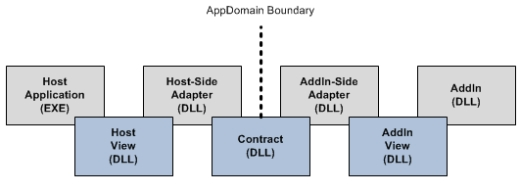
\includegraphics[width=12cm]{System_AddIn_Pipeline.jpg}
    \caption{Схема {\tt Add-in pipeline} в {\tt System.Addin}}
    \label{addin_pipeline-scheme}
\end{figure}

Рассмотрим внутренние компоненты {\tt Add-in pipeline}:

\begin{itemize}

  \item Контракт. Как видно из рисунка, контракт представляет собой интерфейс, <<протокол взаимодействия>> хоста и расширения, и является точкой их соприкосновения;

  \item Далее по обе стороны контракта создаются адаптеры (наследуют {\tt Views}), которые реализуют соответствующие классы представления ({\tt Views}) и оборачивают контракт интерфейсом, который предоставляет {\tt view};

  \item Классы-представления. Они являются соответствующими представлениями типов и методов, которые используются при взаимодействии хоста и расширения.

\end{itemize}

На рисунке \ref{addin_multiple-scheme} представлена схема взаимодействия хост-приложения и плагинов при помощи {\tt Add-in pipeline}.

\begin{figure}[!h]
    \centering
    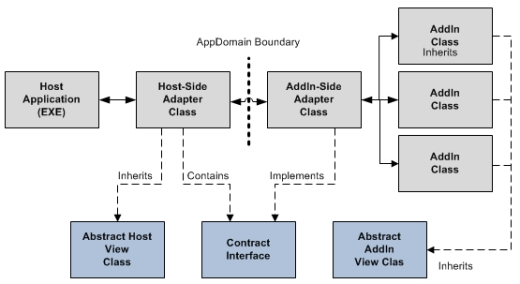
\includegraphics[width=12cm]{System_AddIn_Multiple.jpg}
    \caption{Схема взаимодействия хост-приложения с несколькими плагинами через {\tt Add-in pipeline} в {\tt System.Addin}}
    \label{addin_multiple-scheme}
\end{figure}

Стоит также отметить, что архитектура накладывает некоторые ограничения:
\begin{itemize}

  \item Каждый сегмент из конвейера представляет собой отдельную сборку. Представления можно объединить в одну сборку, но только при условии такого же объединения адаптеров;

  \item {\tt Addin}-ы, адаптеры и контракты должны быть публичны и помечены специальными атрибутами;

  \item Требуется соблюдение жёсткой структуры папок, которая должна строго соблюдаться для нормального функционирования конвейера;

  \item Так как наиболее типичным является сценарий с активацией расширения в отдельном домене, то при проектировании не стоит забывать о том, что пересекающие границы доменов(в качестве параметров или возвращаемых значений) объекты должны быть сериализуемы.

\end{itemize}
